\let\negmedspace\undefined
\let\negthickspace\undefined
\documentclass[journal,12pt,twocolumn]{IEEEtran}

\usepackage{cite}
\usepackage{amsmath,amssymb,amsfonts,amsthm}
\usepackage{algorithmic}
\usepackage{graphicx}
\usepackage{textcomp}
\usepackage{xcolor}
\usepackage{txfonts}
\usepackage{listings}
\usepackage{enumitem}
\usepackage{mathtools}
\usepackage{gensymb}
\usepackage[breaklinks=true]{hyperref}
\usepackage{tkz-euclide} % loads  TikZ and tkz-base
\usepackage{listings}
\usepackage{circuitikz}
\usepackage{graphicx}

%\newcounter{MYtempeqncnt}
\DeclareMathOperator*{\Res}{Res}
%\renewcommand{\baselinestretch}{2}
\renewcommand\thesection{\arabic{section}}
\renewcommand\thesubsection{\thesection.\arabic{subsection}}
\renewcommand\thesubsubsection{\thesubsection.\arabic{subsubsection}}

\renewcommand\thesectiondis{\arabic{section}}
\renewcommand\thesubsectiondis{\thesectiondis.\arabic{subsection}}
\renewcommand\thesubsubsectiondis{\thesubsectiondis.\arabic{subsubsection}}

% correct bad hyphenation here
\hyphenation{op-tical net-works semi-conduc-tor}
\def\inputGnumericTable{}                                 %%

\lstset{
	frame=single,
	breaklines=true,
	columns=fullflexible
}



\newtheorem{theorem}{Theorem}[section]
\newtheorem{problem}{Problem}
\newtheorem{proposition}{Proposition}[section]
\newtheorem{lemma}{Lemma}[section]
\newtheorem{corollary}[theorem]{Corollary}
\newtheorem{example}{Example}[section]
\newtheorem{definition}[problem]{Definition}
\newcommand{\BEQA}{\begin{eqnarray}}
	\newcommand{\EEQA}{\end{eqnarray}}
\newcommand{\define}{\stackrel{\triangle}{=}}
\newcommand\figref{Fig.~\ref}
\newcommand\tabref{Table~\ref}
\bibliographystyle{IEEEtran}
%\bibliographystyle{ieeetr}


\providecommand{\mbf}{\mathbf}
\providecommand{\pr}[1]{\ensuremath{\Pr\left(#1\right)}}
\providecommand{\qfunc}[1]{\ensuremath{Q\left(#1\right)}}
\providecommand{\sbrak}[1]{\ensuremath{{}\left[#1\right]}}
\providecommand{\lsbrak}[1]{\ensuremath{{}\left[#1\right.}}
\providecommand{\rsbrak}[1]{\ensuremath{{}\left.#1\right]}}
\providecommand{\brak}[1]{\ensuremath{\left(#1\right)}}
\providecommand{\lbrak}[1]{\ensuremath{\left(#1\right.}}
\providecommand{\rbrak}[1]{\ensuremath{\left.#1\right)}}
\providecommand{\cbrak}[1]{\ensuremath{\left\{#1\right\}}}
\providecommand{\lcbrak}[1]{\ensuremath{\left\{#1\right.}}
\providecommand{\rcbrak}[1]{\ensuremath{\left.#1\right\}}}
\theoremstyle{remark}
\newtheorem{rem}{Remark}
\newcommand{\sgn}{\mathop{\mathrm{sgn}}}
\providecommand{\abs}[1]{\left\vert#1\right\vert}
\providecommand{\res}[1]{\Res\displaylimits_{#1}}
\providecommand{\norm}[1]{\left\lVert#1\right\rVert}
%\providecommand{\norm}[1]{\lVert#1\rVert}
\providecommand{\mtx}[1]{\mathbf{#1}}
\providecommand{\mean}[1]{E\left[ #1 \right]}
\providecommand{\fourier}{\overset{\mathcal{F}}{ \rightleftharpoons}}
%\providecommand{\hilbert}{\overset{\mathcal{H}}{ \rightleftharpoons}}
\providecommand{\system}{\overset{\mathcal{H}}{ \longleftrightarrow}}
%\newcommand{\solution}[2]{\textbf{Solution:}{#1}}
\newcommand{\solution}{\noindent \textbf{Solution: }}
\newcommand{\cosec}{\,\text{cosec}\,}
\providecommand{\dec}[2]{\ensuremath{\overset{#1}{\underset{#2}{\gtrless}}}}
\newcommand{\myvec}[1]{\ensuremath{\begin{pmatrix}#1\end{pmatrix}}}
\newcommand{\mydet}[1]{\ensuremath{\begin{vmatrix}#1\end{vmatrix}}}
\renewcommand{\abstractname}{Question}

\let\vec\mathbf

	
	\vspace{3cm}
	
	


\newcommand{\permcomb}[4][0mu]{{{}^{#3}\mkern#1#2_{#4}}}
\newcommand{\comb}[1][-1mu]{\permcomb[#1]{C}}

%\IEEEpeerreviewmaketitle

\newcommand \tab [1][1cm]{\hspace*{#1}}
%\newcommand{\Var}{$\sigma ^2$}
\usepackage{amssymb}
\usepackage{amsmath}
\title{
	
\title{GATE 2023 EC 48}
\author{EE23BTECH11061 - SWATHI DEEPIKA$^{*}$% <-this % stops a space
}


}
\begin{document}

\maketitle

\textbf{Question:} 
Let an input x[n] having discrete time Fourier transform
 $X(e^{j\omega})$  = $1 - e^{-j\omega} + 2e^{-3j\omega}$  be passed through an LTI system. The frequency response of the LTI system is  $H(e^{j\omega})$ = $1 - \frac{1}{2} e^{-2j\omega}$ . The output $y[n]$ of the system is \\  
\solution

 \begin{table}[h]
 	\centering
 	\resizebox{6 cm}{!}{
 		
    \begin{tabular}{|c|c|c|}
    \hline
     \textbf{Symbol} & \textbf{Value} &
     \textbf{Description}\\
    \hline
     $x(n)$ &  $(4n+1)u(n)$ & The nth term of the sequence\\[6pt]
    \hline 
     $x(17)$ &  $?$ & 17nth term \\[6pt]
    \hline
     $x(24)$ &  $?$ & 24th term\\[6pt]
    \hline
     
\end{tabular}

 	}
 	\vspace{6 pt}
 	\caption{Parameters}
 	\label{tab:swag_tabel} 
 \end{table}
 
 \begin{align}
 \delta[n]=\frac{1}{2\pi}\int_{-\infty}^{+\infty} e^{j\omega n} d\omega
 \end{align}
\begin{align}
\delta[n] = \begin{cases} 1 & \text{if } n = 0 \\ 0 & \text{otherwise} \end{cases}
\end{align}
\begin{align}
y[n] &= x[n] * h[n]
\end{align}
\begin{align*}
x(n) * h(n) \longleftrightarrow X(e^{j\omega}) \cdot H(e^{j\omega})
\end{align*}
\begin{align}
Y(e^{j\omega}) &= X(e^{j\omega}) \cdot H(e^{j\omega})
\end{align}
\begin{align}
Y(e^{j\omega}) &= (1 - e^{-j\omega} + 2e^{-3j\omega}) \cdot \left(1 - \frac{1}{2}e^{-2j\omega}\right) \\
&= (1 - e^{-j\omega} + \frac{5}{2}e^{-3j\omega} - \frac{1}{2}e^{-2j\omega} - e^{-5j\omega})
\end{align}
\begin{align*}
y[n] = \mathcal{F}^{-1}\{ Y(e^{j\omega}) \}
\end{align*}
\begin{align}
y[n] &= \frac{1}{2\pi}\int_{-\infty}^{+\infty}  Y(e^{j\omega})e^{j\omega n} d\omega \\
&= \frac{1}{2\pi}\int_{-\infty}^{+\infty}  \left(1 - e^{-j\omega} + \frac{5}{2}e^{-3j\omega} - \frac{1}{2}e^{-2j\omega} - e^{-5j\omega}\right)e^{j\omega n} d\omega \\
&= \frac{1}{2\pi}\int_{-\infty}^{+\infty} e^{j\omega n} d\omega - \frac{1}{2\pi}\int_{-\infty}^{+\infty} e^{j\omega(n-1)} d\omega +\frac{1}{2\pi}\int_{-\infty}^{+\infty} \frac{5}{2}e^{j\omega (n-3)} d\omega 
- \frac{1}{2\pi}\int_{-\infty}^{+\infty} \frac{1}{2}e^{j\omega (n-2)} d\omega - \frac{1}{2\pi}\int_{-\infty}^{+\infty} e^{j\omega (n-5)} d\omega 
\end{align}

\begin{align}
 y[n] &= \delta[n] - \delta[n-1] + \frac{5}{2}\delta[n-3] - \frac{1}{2}\delta[n-2] - \delta[n-5]
\end{align}

\begin{align}
y[n] = \delta[n] - \delta[n-1] + 2.5\delta[n-3] - 0.5\delta[n-2] - \delta[n-5] 
\end{align}

\begin{figure}[!h]
    \centering
    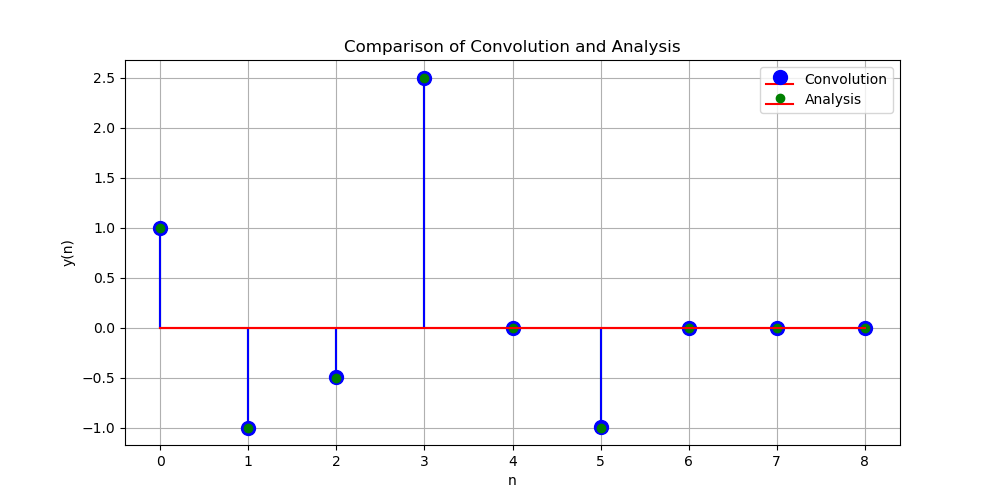
\includegraphics[width = \columnwidth]{figs/plotsss.png}
    \caption{$y(n)$ vs $n$}
    \label{fig:swag_plot}
\end{figure}




\end{document}




